

\newcommand{\yerithpgisystemdaemon}{YERITH--PGI--$9.0$--SYSTEM--DAEMON\xspace}

\newcommand{\elementgraphique}[1]{"\texttt{#1}"\xspace}

\newcommand{\manager}{\emph{Manager}\xspace}
\newcommand{\gestionairedestocks}{\emph{GestionaireDeStocks}\xspace}
\newcommand{\magasinier}{\emph{Magasinier}\xspace}
\newcommand{\caissier}{\emph{Caissier}\xspace}
\newcommand{\vendeur}{\emph{Vendeur}\xspace}
\newcommand{\administrateur}{\emph{Administrateur}\xspace}

\newcommand{\managerb}{\emph{\textbf{Manager}}\xspace}
\newcommand{\gestionairedestocksb}{\emph{\textbf{GestionaireDeStocks}}\xspace}
\newcommand{\vendeurb}{\emph{\textbf{Vendeur}}\xspace}
\newcommand{\caissierb}{\emph{\textbf{Caissier}}\xspace}
\newcommand{\administrateurb}{\emph{\textbf{Administrateur}}\xspace}


\chapter{\yrCOLORgold{Brief Overview of Configuration Data for \yeritherp}}

\YERITHCHAPINTRO{
	\yremphsc{This chapter shows a structure view of how
	configuration data for \yeritherp are organized.}
}


\vspace*{1.05em}


\begin{center}
\captionof{figure}{\yremphscBF{Screenshot of configuration data in administrative section of \yeritherp.}}
\yriLabelFORTABLEFigureWITHvspace{0.00em}{fig:gdebi-gtk-user-graphical-interface}
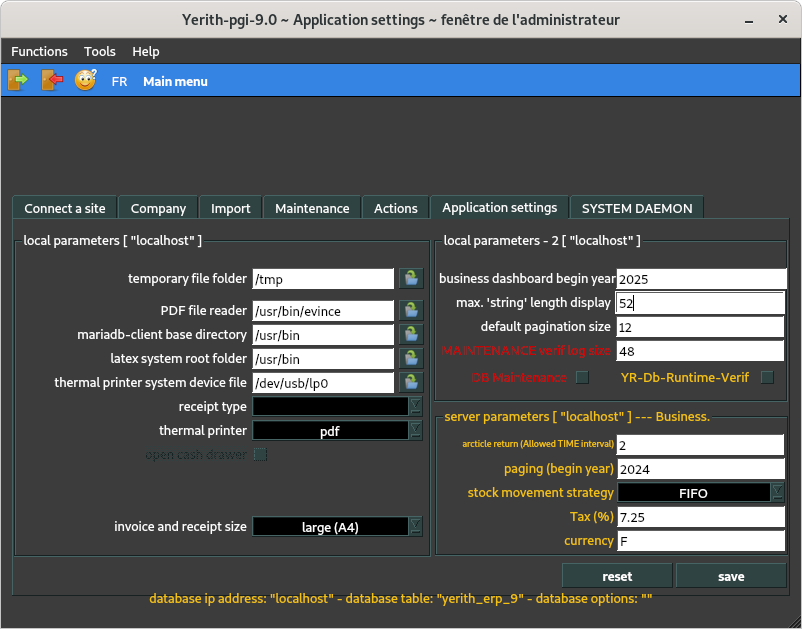
\includegraphics[scale=0.60]{images/Yerith-Erp-Pgi-9-0-Screenshot-configurations-data-Administrative-section.png}
\end{center}


\vspace*{0.95em}



\section{INTRODUCTION}
\index{paramètres locaux}
\index{paramètres serveurs}

\vspace*{1em}

\begin{table*}[!htbp]
\centering
\captionof{table}{Types de paramètres de l'application PGI yeritherp et 
	du système d’alertes et de sauvegardes automatisées.}
\label{tab:parametres-de-lapplication-pgi}
%\resizebox{\textwidth}{!}{%to fit the table within the text width
\begin{tabular}{|c|c|} \hline

\textbf{TYPES DE PARAMÈTRES} 	& 
\textbf{UTILISATEURS MODIFICATEURS}			\\ \hline

paramètres locaux					&
\administrateur, \manager			\\ \hline
		
paramètres serveurs					&
\manager							\\ \hline		

\end{tabular}
%}
\end{table*}

\vspace*{1em}

Tous les paramètres du PGI yeritherp sont
centralisés dans la section \elementgraphique{ADMINISTRATION}.	

Il existe des \textbf{paramètres locaux}
(enregistrés sur le disque dur de l'ordinateur
de l’utilisateur), et des \textbf{paramètres serveurs}
(enregistrés dans la base de données du PGI
yeritherp):

\begin{enumerate}[1.]
	\item Des \textbf{paramètres locaux} influencent
		uniquement des instances du PGI 
		yeritherp dans l'ordinateur de
		l’utilisateur, et sont modifiables par 
		$1$ \administrateurb ou $1$ \managerb.
		
	\item Des \textbf{paramètres serveurs} influencent
		TOUTES LES INSTANCES DU PGI yeritherp
		QUI SONT RATTACHÉES AU SERVEUR DE BASE
		DE DONNÉES EN QUESTION !
		
		Des paramètres serveurs sont modifiables
		UNIQUEMENT par $1$ \managerb.
\end{enumerate}

Tous les types de paramètres et les utilisateurs
responsables de leurs modifications sont illustrés
dans le TABLEAU~\ref{tab:parametres-de-lapplication-pgi}.\\


TOUS PARAMÈTRE LOCAL OU SERVEUR EST SOIT:
\begin{enumerate}[1.]
	\item \emphbf{$1$ paramètre de l'application erp (pgi)}
			(SECTION~\ref{subsec:parametres-de-lapplication-erp-pgi})
	\item \emphbf{$1$ paramètre du système d’alertes et
		de sauvegardes automatisées}
		(SECTION~\ref{subsec:parametres-du-systeme-dalerte-et-de-sauvegarde-automatisee}).
\end{enumerate}


\newpage


\section{PARAMÈTRES DE L'APPLICATION ERP (PGI)}
\index{paramètres de l’application erp (pgi) yeritherp}
\label{subsec:parametres-de-lapplication-erp-pgi}

\vspace*{1em}

\begin{center}
\captionof{figure}{La fen\^etre de paramétrage du PGI yeritherp.}
\label{fig:fenetre-de-visualisation-du-PGI-yerith-erp-9-0}
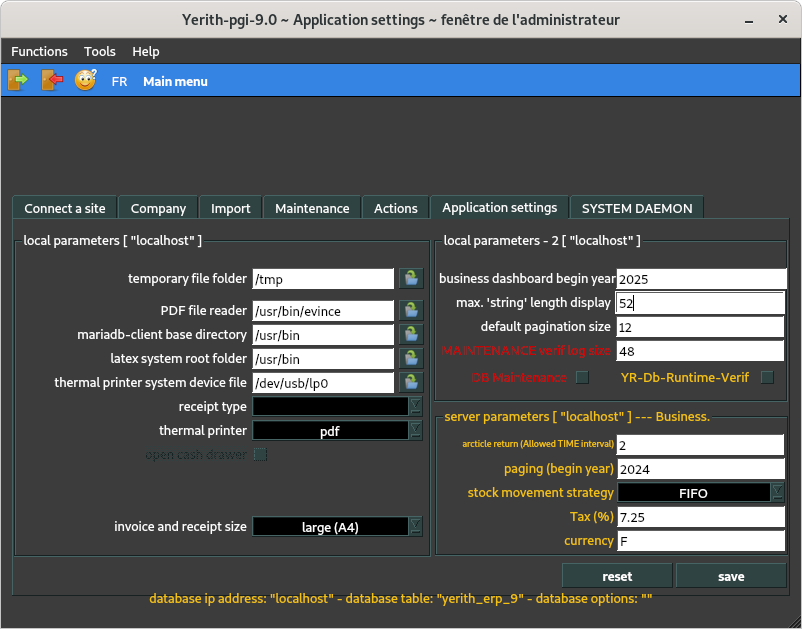
\includegraphics[scale=0.5]{images/Yerith-Erp-Pgi-9-0-Screenshot-configurations-data-Administrative-section.png}
\end{center}

\vspace*{1em}

$1$ paramètre de l’application erp (pgi) yeritherp
est $1$ valeur qui influence ses comportements
du PGI yeritherp lors de son exécution:
\emphbf{le format des reçus ("\emphbf{petit}",
"\emphbf{A$4$}", ou "\emphbf{A$5$}") en est $1$ exemple !}




\subsection{LOCAL parameters --- Computer LOCAL specific}



\subsection{\yrCOLORDarkorange{Server parameters --- BUSINESS--only correlated information}}




\newpage


\section{PARAMÈTRES DU SYSTÈME D'ALERTES ET DE SAUVEGARDE AUTOMATISÉE DE LA
			BASE DE DONNÉES}
\index{paramètres du système d'alertes, et du
	système de sauvegarde automatisée \yerithpgisystemdaemon}
\label{subsec:parametres-du-systeme-dalerte-et-de-sauvegarde-automatisee}

\vspace*{1em}

\begin{center}
\captionof{figure}{La fen\^etre de paramétrage du système d'alertes,
			et du système de sauvegarde automatisée.}
\label{fig:fenetre-de-visualisation-du-systeme-dalerte}
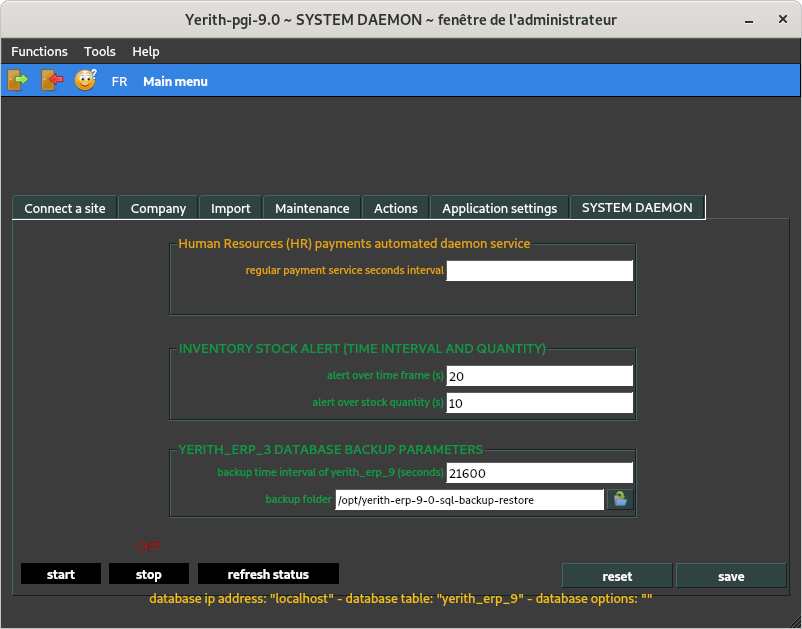
\includegraphics[scale=0.5]{images/yerith-erp-9-0-system-daemon-parameters.png}
\end{center}

\vspace*{1em}

$1$ paramètre du système d'alertes, et du système
de sauvegarde automatisée \yerithpgisystemdaemon est
$1$ valeur qui influence ses comportements lors
de son exécution: \emphbf{le répertoire de sauvegarde des
bases de données \mysql de yeritherp EN EST $1$ EXEMPLE !} 




